% Written by Anders Sjoqvist and Ulf Lundstrom, 2009
% The main sources are: tinyKACTL, Beta and Wikipedia

\chapter{Mathematics}

\section{Recurrences}
If $a_n = c_1 a_{n-1} + \dots + c_k a_{n-k}$, and $r_1, \dots, r_k$ are distinct roots of $x^k + c_1 x^{k-1} + \dots + c_k$, there are $d_1, \dots, d_k$ s.t.
\[a_n = d_1r_1^n + \dots + d_kr_k^n. \]
Non-distinct roots $r$ become polynomial factors, e.g. $a_n = (d_1n + d_2)r^n$.

\section{Trigonometry}
\begin{align*}
\sin(v+w)&{}=\sin v\cos w+\cos v\sin w\\
cos(v+w)&{}=\cos v\cos w-\sin v\sin w\\
\end{align*}
\begin{align*}
\tan(v+w)&{}=\dfrac{\tan v+\tan w}{1-\tan v\tan w}\\
\sin v+\sin w&{}=2\sin\dfrac{v+w}{2}\cos\dfrac{v-w}{2}\\
\cos v+\cos w&{}=2\cos\dfrac{v+w}{2}\cos\dfrac{v-w}{2}
\end{align*}
\[ (V+W)\tan(v-w)/2{}=(V-W)\tan(v+w)/2 \]
where $V, W$ are lengths of sides opposite angles $v, w$.
\begin{align*}
	a\cos x+b\sin x&=r\cos(x-\phi)\\
	a\sin x+b\cos x&=r\sin(x+\phi)
\end{align*}
where $r=\sqrt{a^2+b^2}, \phi=\operatorname{atan2}(b,a)$.

\section{Geometry}

\subsection{Triangles}
Side lengths: $a,b,c$\\
Semiperimeter: $p=\dfrac{a+b+c}{2}$\\
Area: $A=\sqrt{p(p-a)(p-b)(p-c)}$\\
Circumradius: $R=\dfrac{abc}{4A}$\\
Inradius: $r=\dfrac{A}{p}$\\
Length of median (divides triangle into two equal-area triangles): $m_a=\tfrac{1}{2}\sqrt{2b^2+2c^2-a^2}$\\
Length of bisector (divides angles in two): $s_a=\sqrt{bc\left[1-\left(\dfrac{a}{b+c}\right)^2\right]}$\\
Law of sines: $\dfrac{\sin\alpha}{a}=\dfrac{\sin\beta}{b}=\dfrac{\sin\gamma}{c}=\dfrac{1}{2R}$\\
Law of cosines: $a^2=b^2+c^2-2bc\cos\alpha$\\
Law of tangents: $\dfrac{a+b}{a-b}=\dfrac{\tan\dfrac{\alpha+\beta}{2}}{\tan\dfrac{\alpha-\beta}{2}}$\\

\subsection{Spherical coordinates}
\centerline{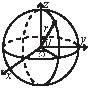
\includegraphics[width=25mm]{../content/math/sphericalCoordinates}}
\[\begin{array}{cc}
x = r\sin\theta\cos\phi & r = \sqrt{x^2+y^2+z^2}\\
y = r\sin\theta\sin\phi & \theta = \textrm{acos}(z/\sqrt{x^2+y^2+z^2})\\
z = r\cos\theta & \phi = \textrm{atan2}(y,x)
\end{array}\]

\section{Derivatives/Integrals}
\begin{align*}
	\dfrac{d}{dx}\arcsin x = \dfrac{1}{\sqrt{1-x^2}} &&& \dfrac{d}{dx}\arccos x = -\dfrac{1}{\sqrt{1-x^2}} \\
	\dfrac{d}{dx}\tan x = 1+\tan^2 x &&& \dfrac{d}{dx}\arctan x = \dfrac{1}{1+x^2} \\
	\int\tan ax = -\dfrac{\ln|\cos ax|}{a} &&& \int x\sin ax = \dfrac{\sin ax-ax \cos ax}{a^2} \\
	\int e^{-x^2} = \frac{\sqrt \pi}{2} \text{erf}(x) &&& \int xe^{ax}dx = \frac{e^{ax}}{a^2}(ax-1)
\end{align*}

Integration by parts:
\[\int_a^bf(x)g(x)dx = [F(x)g(x)]_a^b-\int_a^bF(x)g'(x)dx\]

\section{Sums}
\[ c^a + c^{a+1} + \dots + c^{b} = \frac{c^{b+1} - c^a}{c-1}, c \neq 1 \]
\begin{align*}
	1 + 2 + 3 + \dots + n &= \frac{n(n+1)}{2} \\
	1^2 + 2^2 + 3^2 + \dots + n^2 &= \frac{n(2n+1)(n+1)}{6} \\
	1^3 + 2^3 + 3^3 + \dots + n^3 &= \frac{n^2(n+1)^2}{4} \\
	1^4 + 2^4 + 3^4 + \dots + n^4 &= \frac{n(n+1)(2n+1)(3n^2 + 3n - 1)}{30} \\
\end{align*}

\section{Series} 
$$e^x = 1+x+\frac{x^2}{2!}+\frac{x^3}{3!}+\dots,\,(-\infty<x<\infty)$$
$$\ln(1+x) = x-\frac{x^2}{2}+\frac{x^3}{3}-\frac{x^4}{4}+\dots,\,(-1<x\leq1)$$
$$\sqrt{1+x} = 1+\frac{x}{2}-\frac{x^2}{8}+\frac{2x^3}{32}-\frac{5x^4}{128}+\dots,\,(-1\leq x\leq1)$$
$$\sin x = x-\frac{x^3}{3!}+\frac{x^5}{5!}-\frac{x^7}{7!}+\dots,\,(-\infty<x<\infty)$$
$$\cos x = 1-\frac{x^2}{2!}+\frac{x^4}{4!}-\frac{x^6}{6!}+\dots,\,(-\infty<x<\infty)$$
